\documentclass[12pt]{article}
\usepackage[utf8]{inputenc}

%%% I added a few packages. This next one allows you to set the margins.
\usepackage[top=.5in,bottom=1in,right=.75in,left=.75in]{geometry}
\usepackage{multicol}
%\usepackage{newspaper}
\setlength{\columnsep}{1cm}
\usepackage{blindtext}
\usepackage{varwidth}

%%% This one does boxes in a really nice way.
\usepackage{tcolorbox}
\usepackage{mdframed}
\usepackage{minibox}
\usepackage{graphicx}
\graphicspath{ {./images/} }
\usepackage{epstopdf}
  \epstopdfDeclareGraphicsRule{.pdf}{png}{.png}{convert #1 \OutputFile}
  \DeclareGraphicsExtensions{.png,.pdf}
\usepackage{hyperref}
\hypersetup{
    colorlinks=true,
    linkcolor=blue,
    filecolor=magenta,      
    urlcolor=cyan,
    pdftitle={MSCSMess},
    pdfpagemode=FullScreen,
    }
\urlstyle{same}
 \usepackage{fix-cm}
 \usepackage{soul}
 \usepackage{graphicx}
 \usepackage{multicol}


\newcommand{\ds}{\displaystyle}
\newcommand{\ZZ}{\mathbb{Z}}
\newcommand{\QQ}{\mathbb{Q}}
\newcommand{\RR}{\mathbb{R}}
\newcommand{\CC}{\mathbb{C}}
\newcommand{\FF}{\mathbb{F}}
\newcommand{\xx}{\mathbf{x}}
\newcommand{\uu}{\mathbf{u}}
\newcommand{\vv}{\mathbf{v}}

\newcommand{\bolder}{\textbf}
 
 
\title{\fontsize{60}{70}\selectfont {\bf {MSCS} 
\includegraphics[scale=.3]{images/OleLion.png} {Mess}}}
\author{Department of Mathematics, Statistics, and Computer Science \\ St.\@ Olaf College, Northfield, MN 55057 \vspace{-2ex}} 
\date{\today\, $|$ Volume 54, No.\@ 21 \line(1,0){500}}


\begin{document}

\maketitle \vspace{-1cm}
\begin{center}
Happy Friday everyone! We hope that everyone had an awesome spring break and are ready to get through the rest of the semester. Make sure to take some study breaks and check out the cool events coming up in these next few weeks!

\end{center}

 \begin{multicols}{2}


\begin{tcolorbox}[colback=white, colframe=black]
    \begin{center}
    \title{{\large \bolder{Summer Opportunity in Math Education}}}
    \end{center}
\end{tcolorbox}

\href {https://bsmeducation.com} {Budapest Semesters in Mathematics Education (BSME)} is a 6-week summer program in Budapest, Hungary, designed for those interested in the learning and teaching of mathematics. Participants take a variety of courses in mathematics education and complete a week-long field experience. Come experience the \href{https://bsmeducation.com/wp-content/uploads/2020/02/hungarian-pedagogy-flyer.pdf}{Hungarian pedagogy} based on guided discovery—which emphasizes problem solving, mathematical creativity, and communication—as well as the rich and vibrant culture of Hungary.

Scholarships are available from the St. Olaf Financial Aid Office. See the \href{https://wp.stolaf.edu/smithcenter/st-olaf-summer-programs/#:~:text=All%20students%20are%20automatically%20considered%20for%20a%20need%2Dbased%20scholarship%20(see%20J%2DTerm%20column)%20of%20up%20to%2050%25%20of%20program%20costs%20from%20the%20St.%20Olaf%20Financial%20Aid%20Office.%C2%A0%C2%A0}{Smith Center's} webpage for more details. If you have any questions, contact Prof. Ryota Matsuura (matsuura@stolaf.edu).


 \begin{tcolorbox}[colback=white, colframe=black]
    \begin{center}
    \title{{\large \bolder{Math Education at St. Olaf}}}
    \end{center}
\end{tcolorbox}

At St. Olaf, you can earn a double major in Mathematics and in Education! By taking courses in both departments and completing a student-teaching semester, you can become licensed to teach high school or middle school mathematics after graduation. Given our top-notch program, St. Olaf graduates are highly sought after by schools in Minnesota and beyond.

To learn more about this opportunity, please reach out to Prof. Ryota Matsuura (matsuura@stolaf.edu). See his website \href{https://pages.stolaf.edu/matsuura/math-ed-st-olaf/}{here} for more details, too.

PS: We have a J-term course EDUC 378: Multicultural Education in Hawaii, and yes, it’s an off-campus course!

 \begin{tcolorbox}[colback=white, colframe=black]
    \begin{center}
    \title{{\large \bolder{Annual MSCS Talent Show!}}}
    \end{center}
\end{tcolorbox}
The MSCS Department is hosting the MSCS Recital on Wednesday, April 15th, at 7:00pm in Ytterboe Lounge!

The recital is an annual recognition of the talent (broadly defined), of the members of the MSCS community. Faculty and students will perform, in ensembles or solo, for an hour or two in the evening. Anyone associated with MSCS is welcome to participate, as a performer or an observer. This is a fun, relaxed gathering of students and faculty on equal footing. 

There will be food and drink, including home cooking. If you are interested in performing or have questions, please contact Carlos Chávez (chavez16@stolaf.edu) or Daniel Stoertz (stoert1@stolaf.edu), or fill out \href{https://docs.google.com/forms/d/e/1FAIpQLSctO8sAXxTCjrrDK_F1ocOHFMjC1OTzejShYgvfoWYQjHmg1g/viewform?usp=publish-editor}{this form}.


\begin{tcolorbox}[colback=white, colframe=black]
    \begin{center}
    \title{{\large \bolder{4/20 MSCS Colloquium: Joslenne Peña}}}
    \end{center}
\end{tcolorbox}

Join us for an MSCS Department Colloquium on Monday, April 20th at 3:30pm in RNS 210! Our speaker, Dr. Joslenne Peña (she/her), Assistant Professor of Computer Science at Macalester College, will present "Community Coding Workshops for Life-Long Learners Using Libraries: An Informal Learning Approach". Her talk explores Code for Us (CFU), an NSF-funded program that uses libraries as hubs for teaching foundational programming skills to adult learners. All are welcome!


\begin{tcolorbox}[colback=white, colframe=black]
    \begin{center}
    \title{{\large \bolder{Mario Kart Tournament}}}
    \end{center}
\end{tcolorbox}

Rev your engines! The St. Olaf CS Department is hosting a Mario Kart Tournament on Monday, April 20th at 4:45pm in the CS Advanced Lab. Come for the epic prizes and bring your friends and competitive spirit. Get ready for a splendid time!


\begin{tcolorbox}[colback=white, colframe=black]
    \begin{center}
    \title{{\large \bolder{TLC Lecture: Deanna Haunsperger}}}
    \end{center}
\end{tcolorbox}

Don't miss the TLC Lecture featuring Deanna Haunsperger (she/her) on Friday, April 24th at 3:30pm in RNS 210, with a reception to follow in RNS 207. Her talk, "Halving Your Cake," tackles the age-old question of fair division: how do you split a resource equitably among more than two people? 

Haunsperger is a Professor of Mathematics at Carleton College, past President of the Mathematical Association of America, and co-founder of the Carleton Summer Mathematics Program for Women. We hope you'll stop by!

\begin{tcolorbox}[colback=white, colframe=black]
    \begin{center}
    \title{{\large \bolder{MSCS Grader Applications}}}
    \end{center}
\end{tcolorbox}

The MSCS department is now accepting Grader/TA applications for Fall 2026. If you are interested in working with us please \href{https://forms.gle/c9Rw2DAwuYA8vBtM9}{apply here}. The deadline for applying is Wednesday, April 22nd at 11:59pm. The qualifications are as follows: 

 \begin{itemize}
    \item Completed the course with an A or B.
    \item Ability to maintain confidentiality.
    \item Complete work in a timely manner.
    \item Availability to work the entire semester.
\end{itemize} 

Please contact Melissa Schori (schori1@stolaf.edu) if you have any questions!

\begin{tcolorbox}[colback=white, colframe=black]
    \begin{center}
    \title{{\large \bolder{Computer Science Showcase}}}
    \end{center}
\end{tcolorbox}

Come see what your fellow Oles have been building! The Computer Science Showcase is on Monday, May 11th at 3:30pm in the Buntrock Commons Sun Ballroom. CS students will present their year-long projects, and there will be snacks, good vibes, and prizes up for grabs. Want to show off your own project? Scan the QR code on the poster or reach out to Prof. Leeson (leeson2@stolaf.edu) to sign up.

\vfill\,
 

\begin{tcolorbox}[colback=white, colframe=black]
    \begin{center}
    \title{{\large \bolder{Problem Solving Group}}}
    \end{center}
\end{tcolorbox}
The Math Problem Solving Group meets weekly to have fun, solve math problems, eat candy, and prepare for upcoming math contests. Meetings are Thursdays from 11:30 am - 12:30 pm, in RNS 207 (the Center for Interdisciplinary Research room). Everyone is welcome, regardless of prior experience in mathematics or math contests!


\end{multicols} \vfill 

\begin{center}
    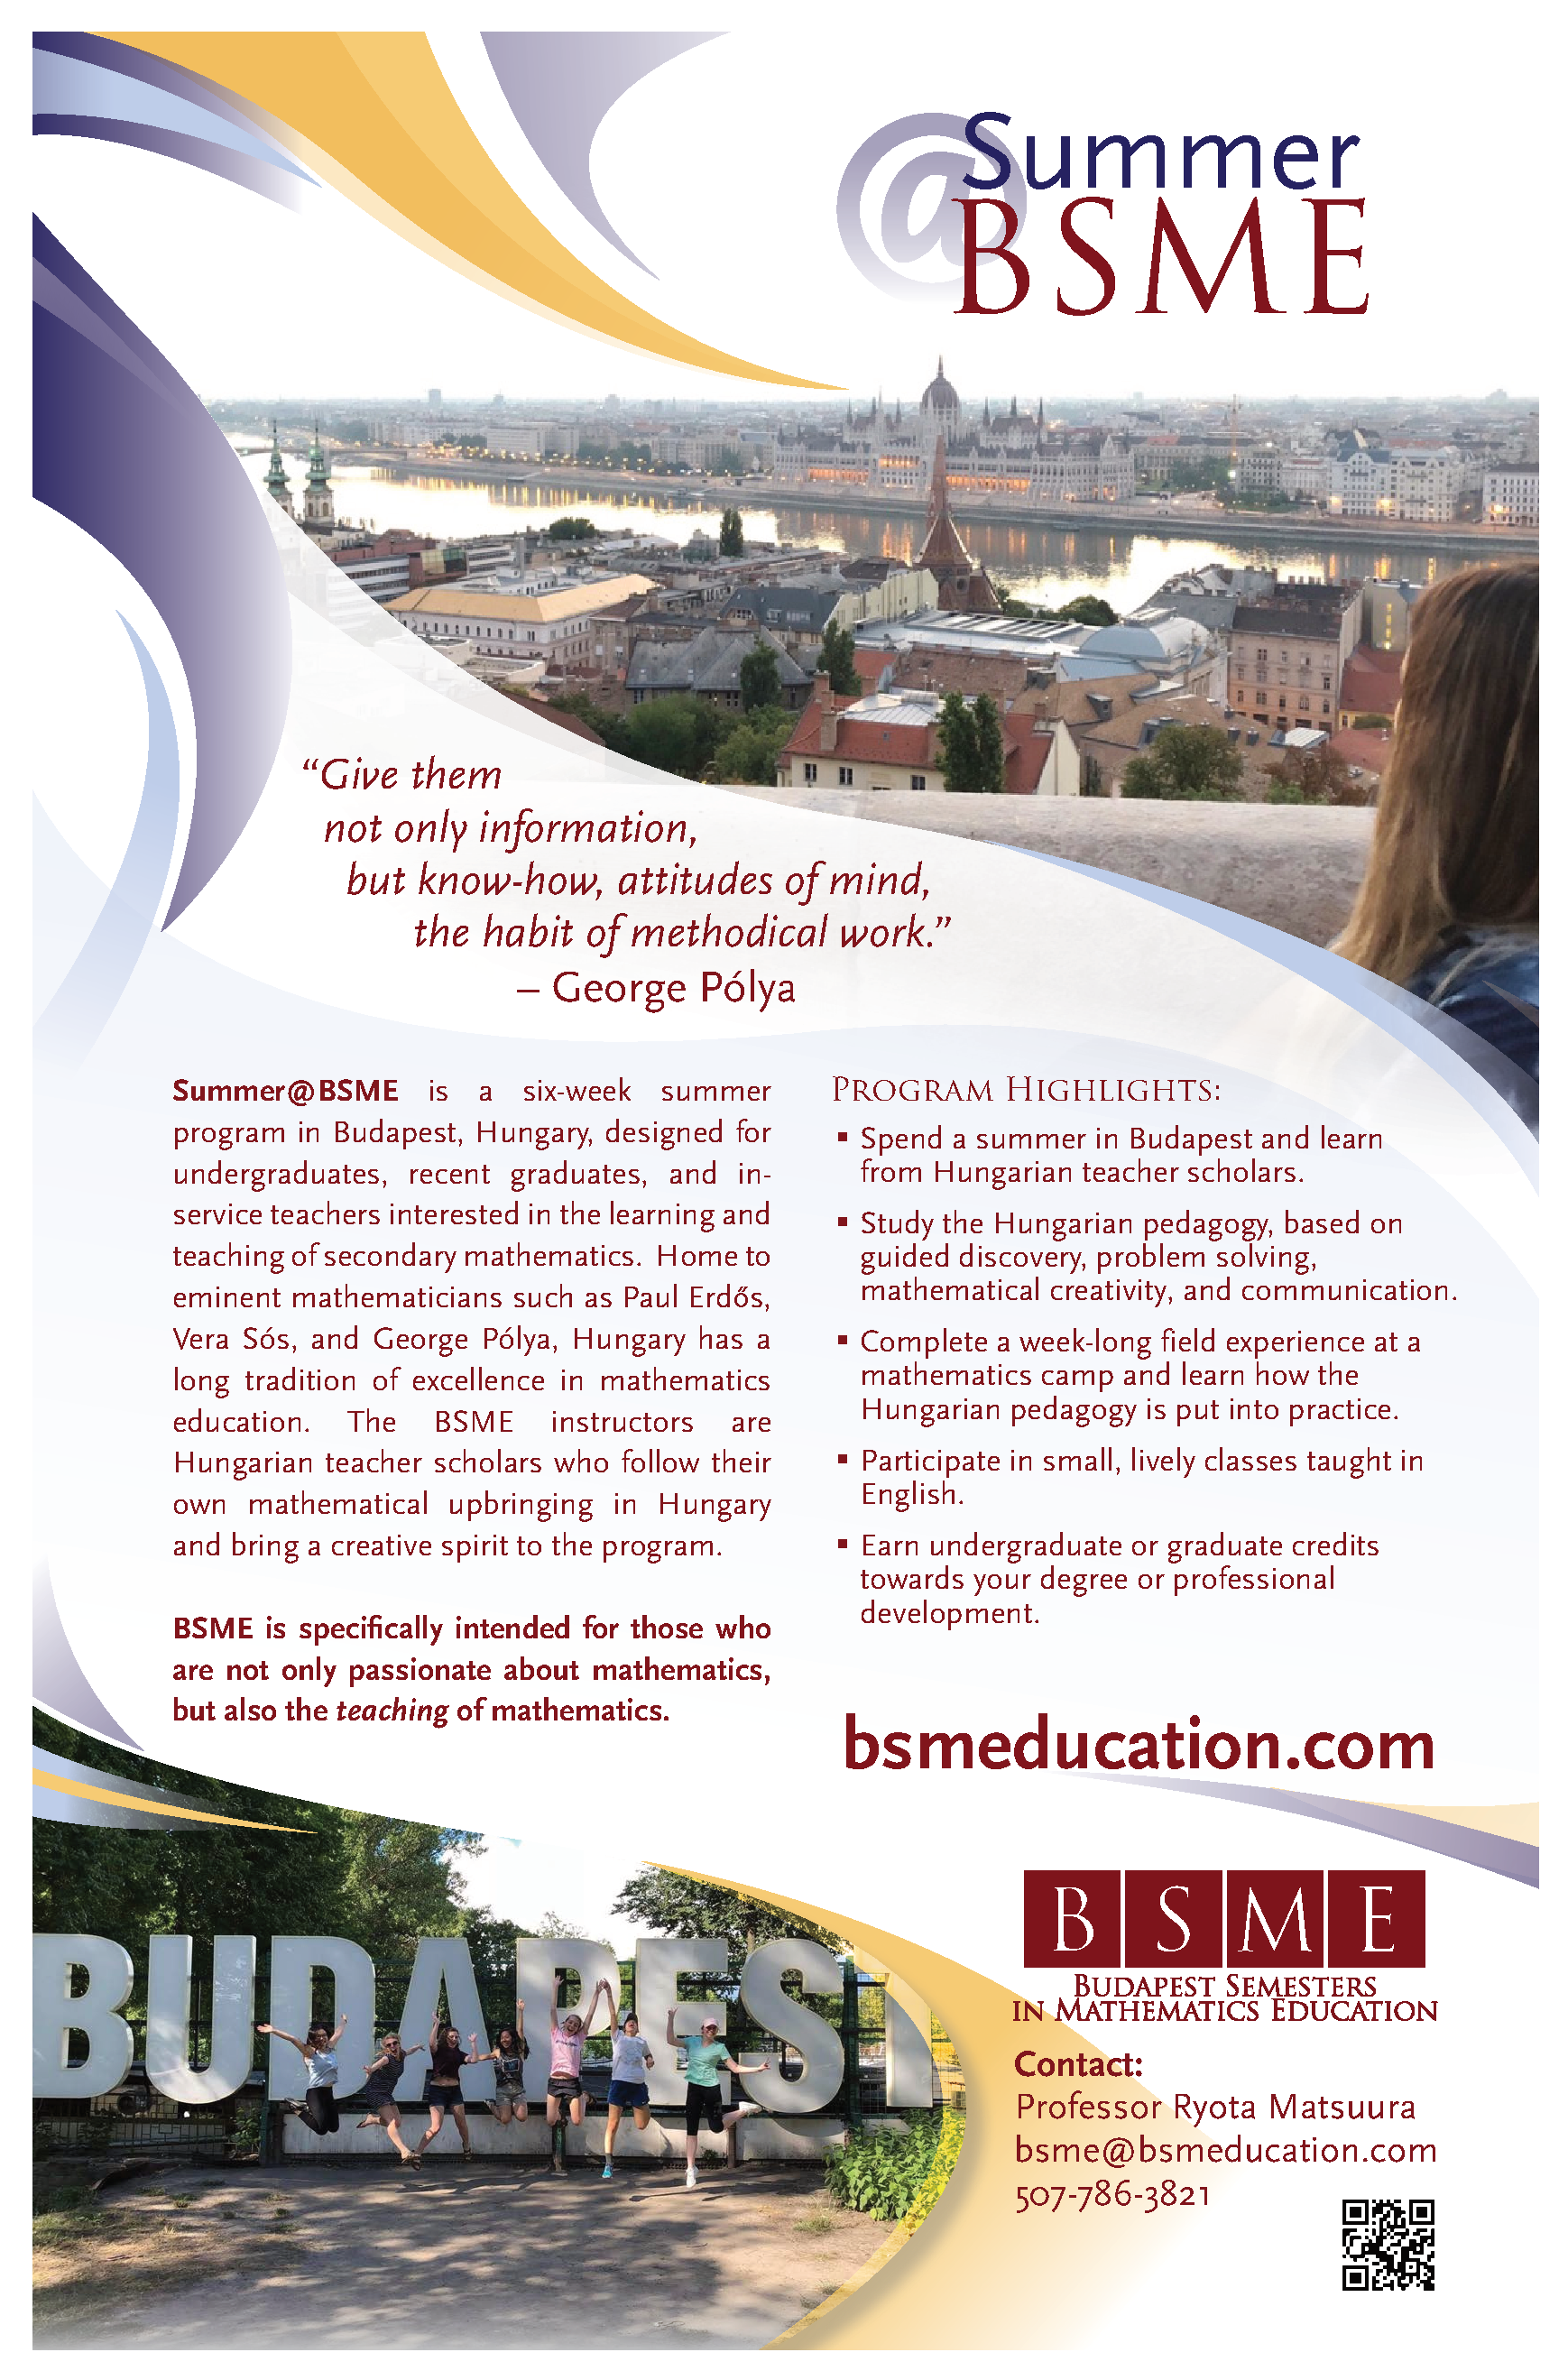
\includegraphics[height=0.95\textheight]{images/2024-bsme-poster-revised-web.pdf}
\end{center}

\begin{center}
    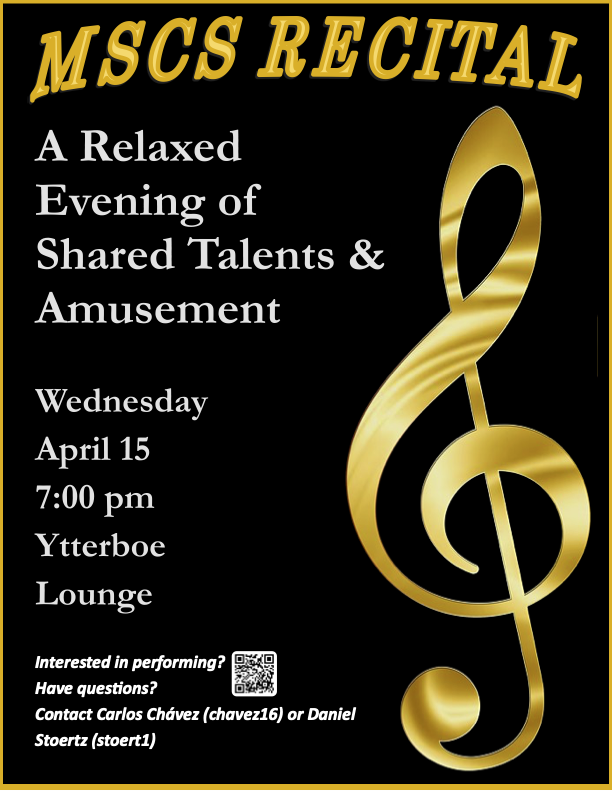
\includegraphics[height=0.95\textheight]{Recital Invite 26_qr.png}
\end{center}

\begin{center}
    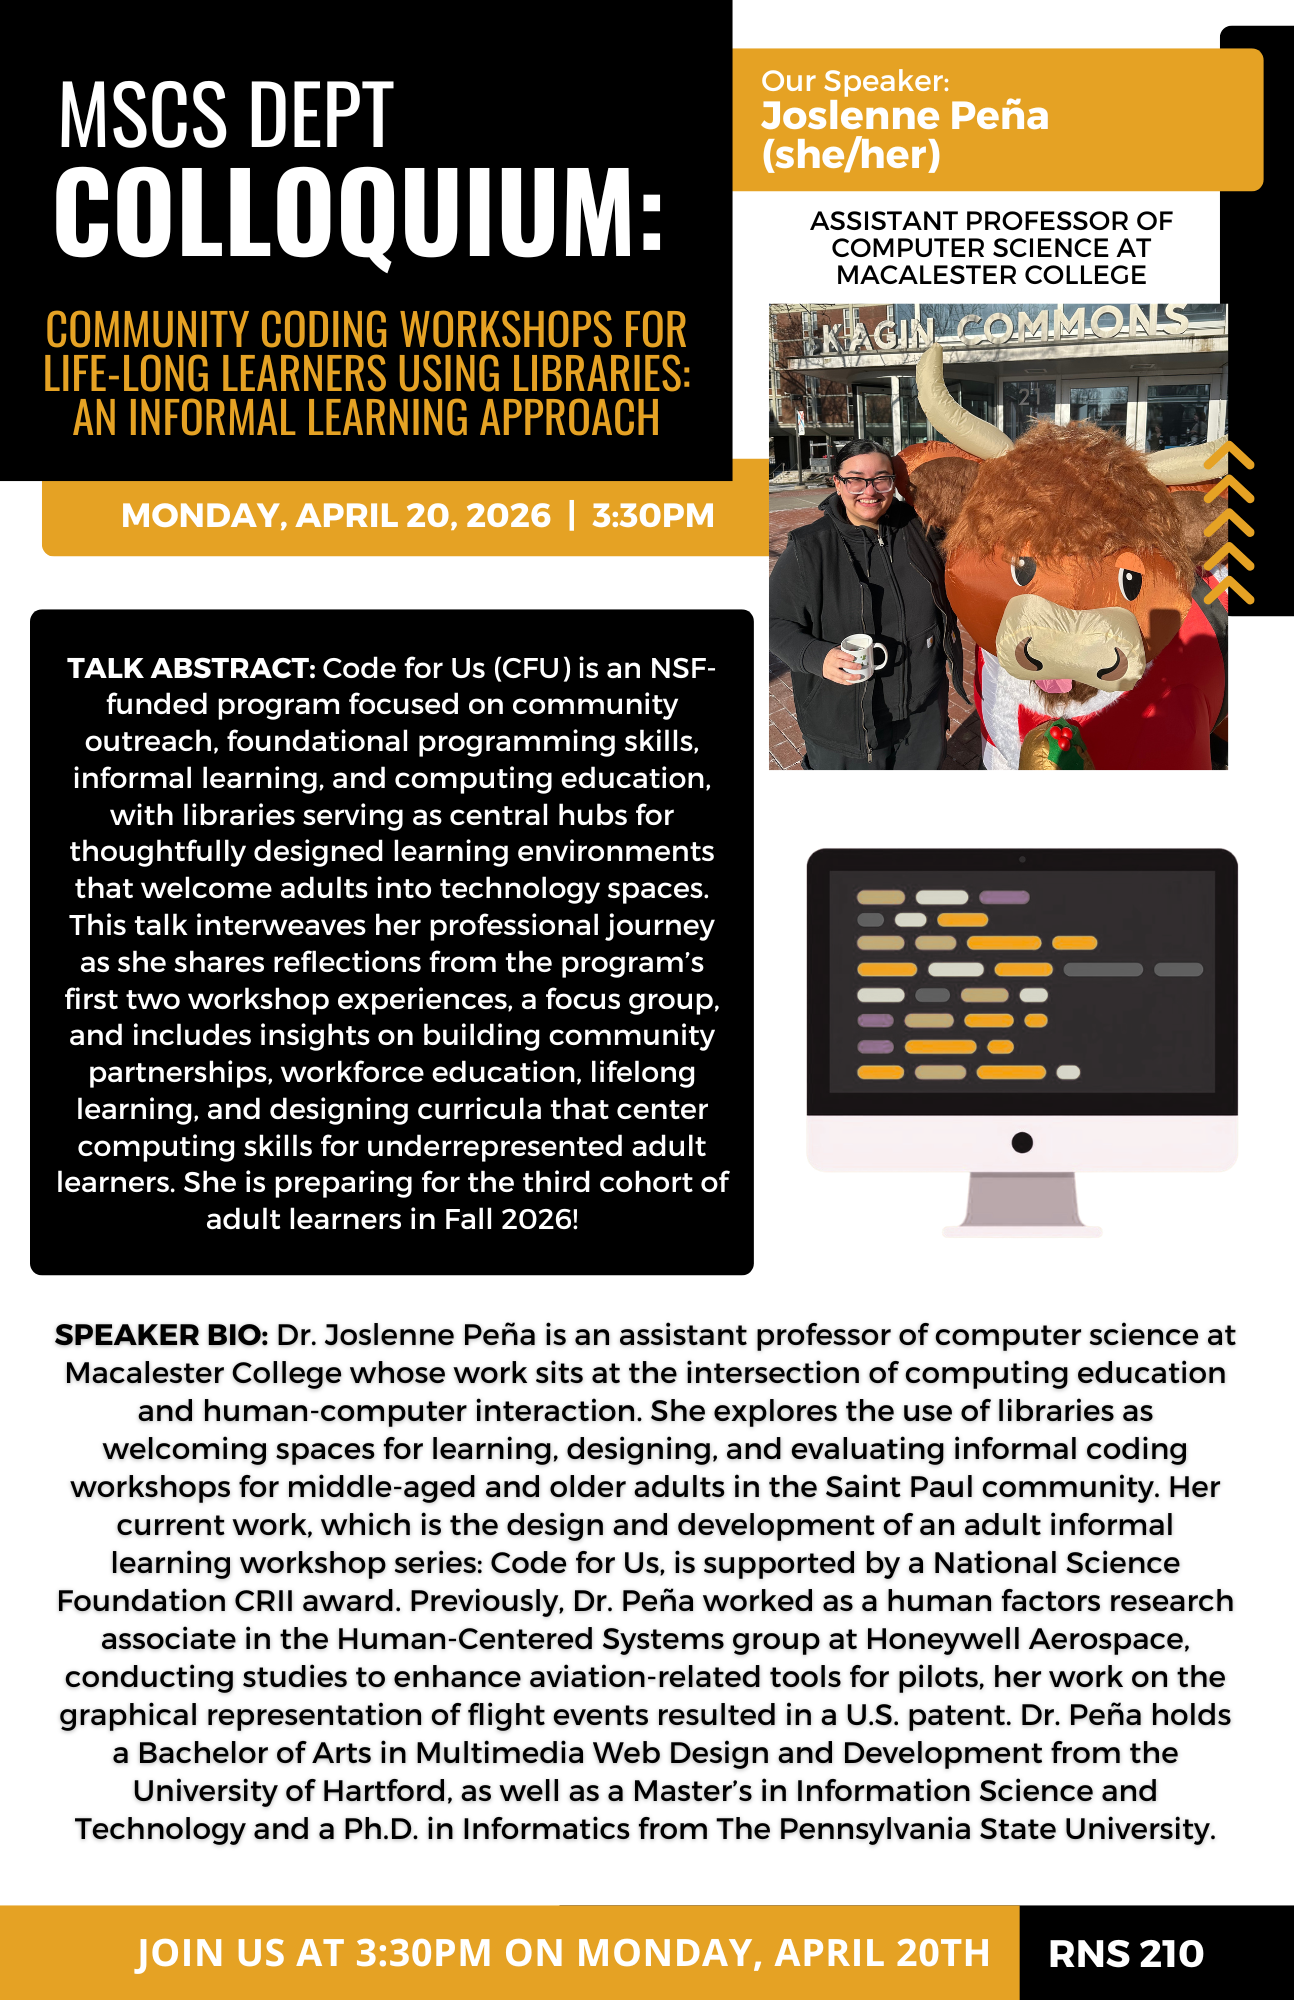
\includegraphics[height=0.95\textheight]{images/Colloquium Joslene Pena.png}
\end{center}

\begin{center}
    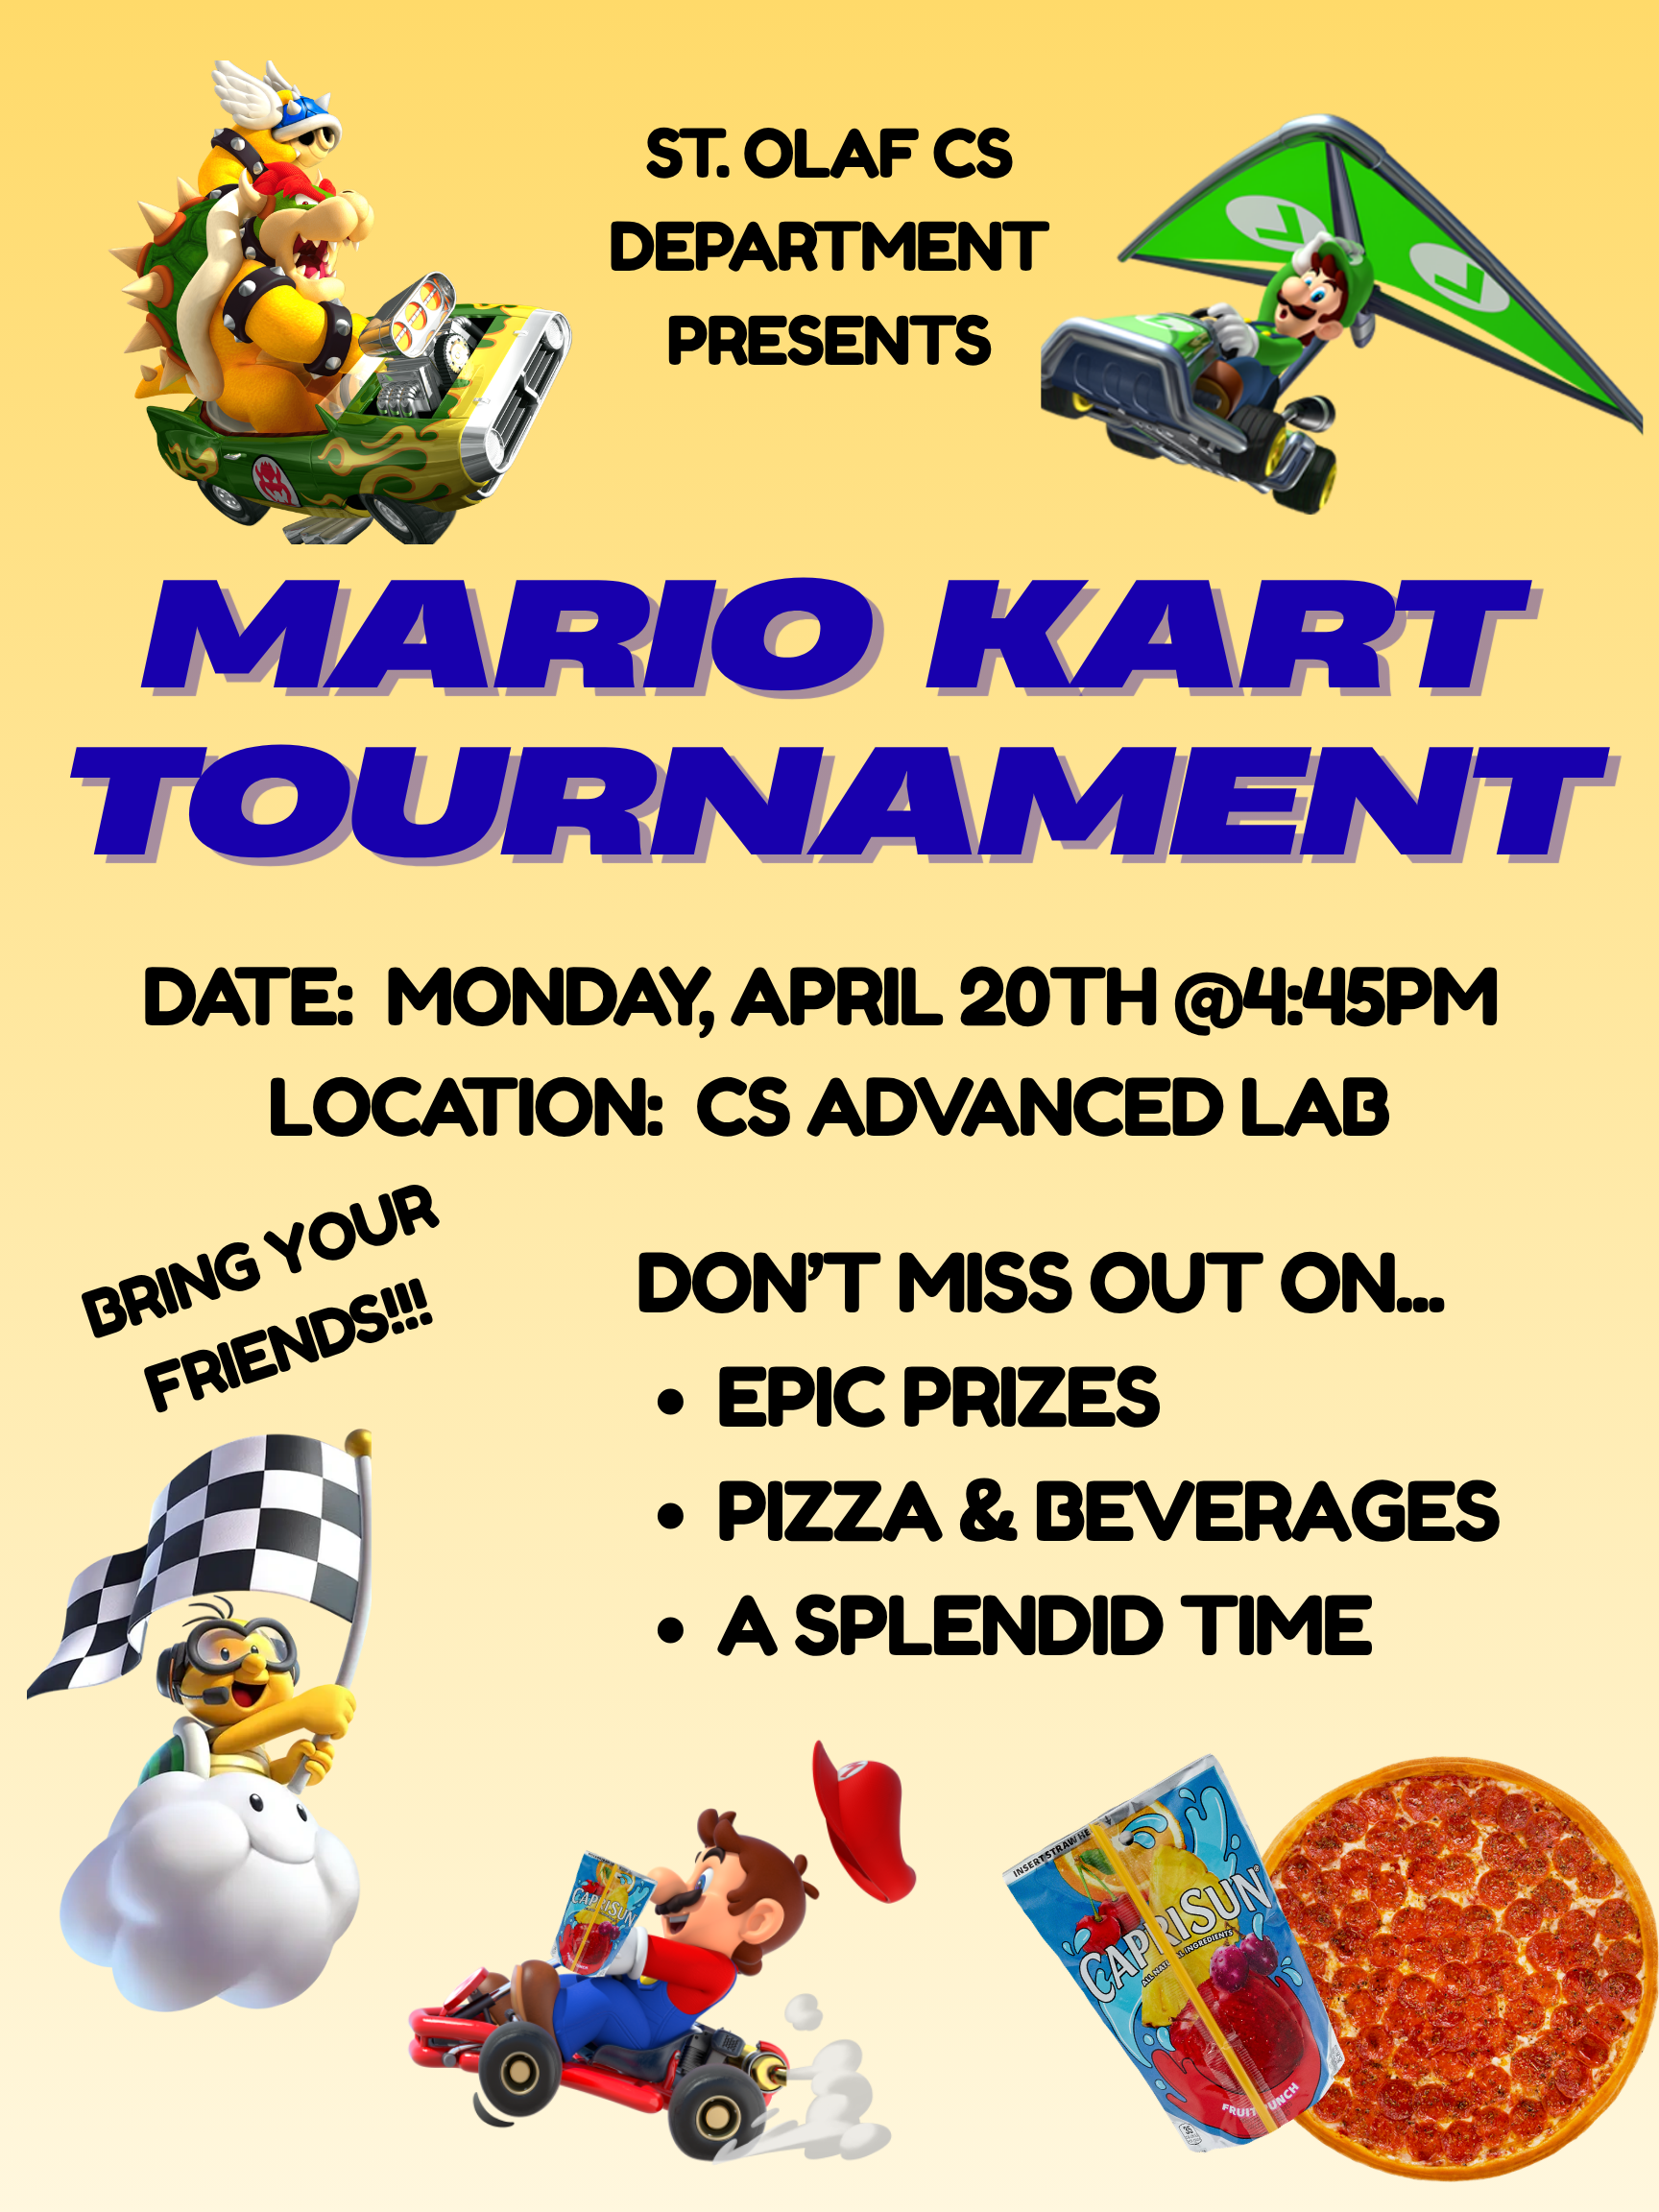
\includegraphics[height=0.95\textheight]{images/MarioKart.png}
\end{center}

\begin{center}
    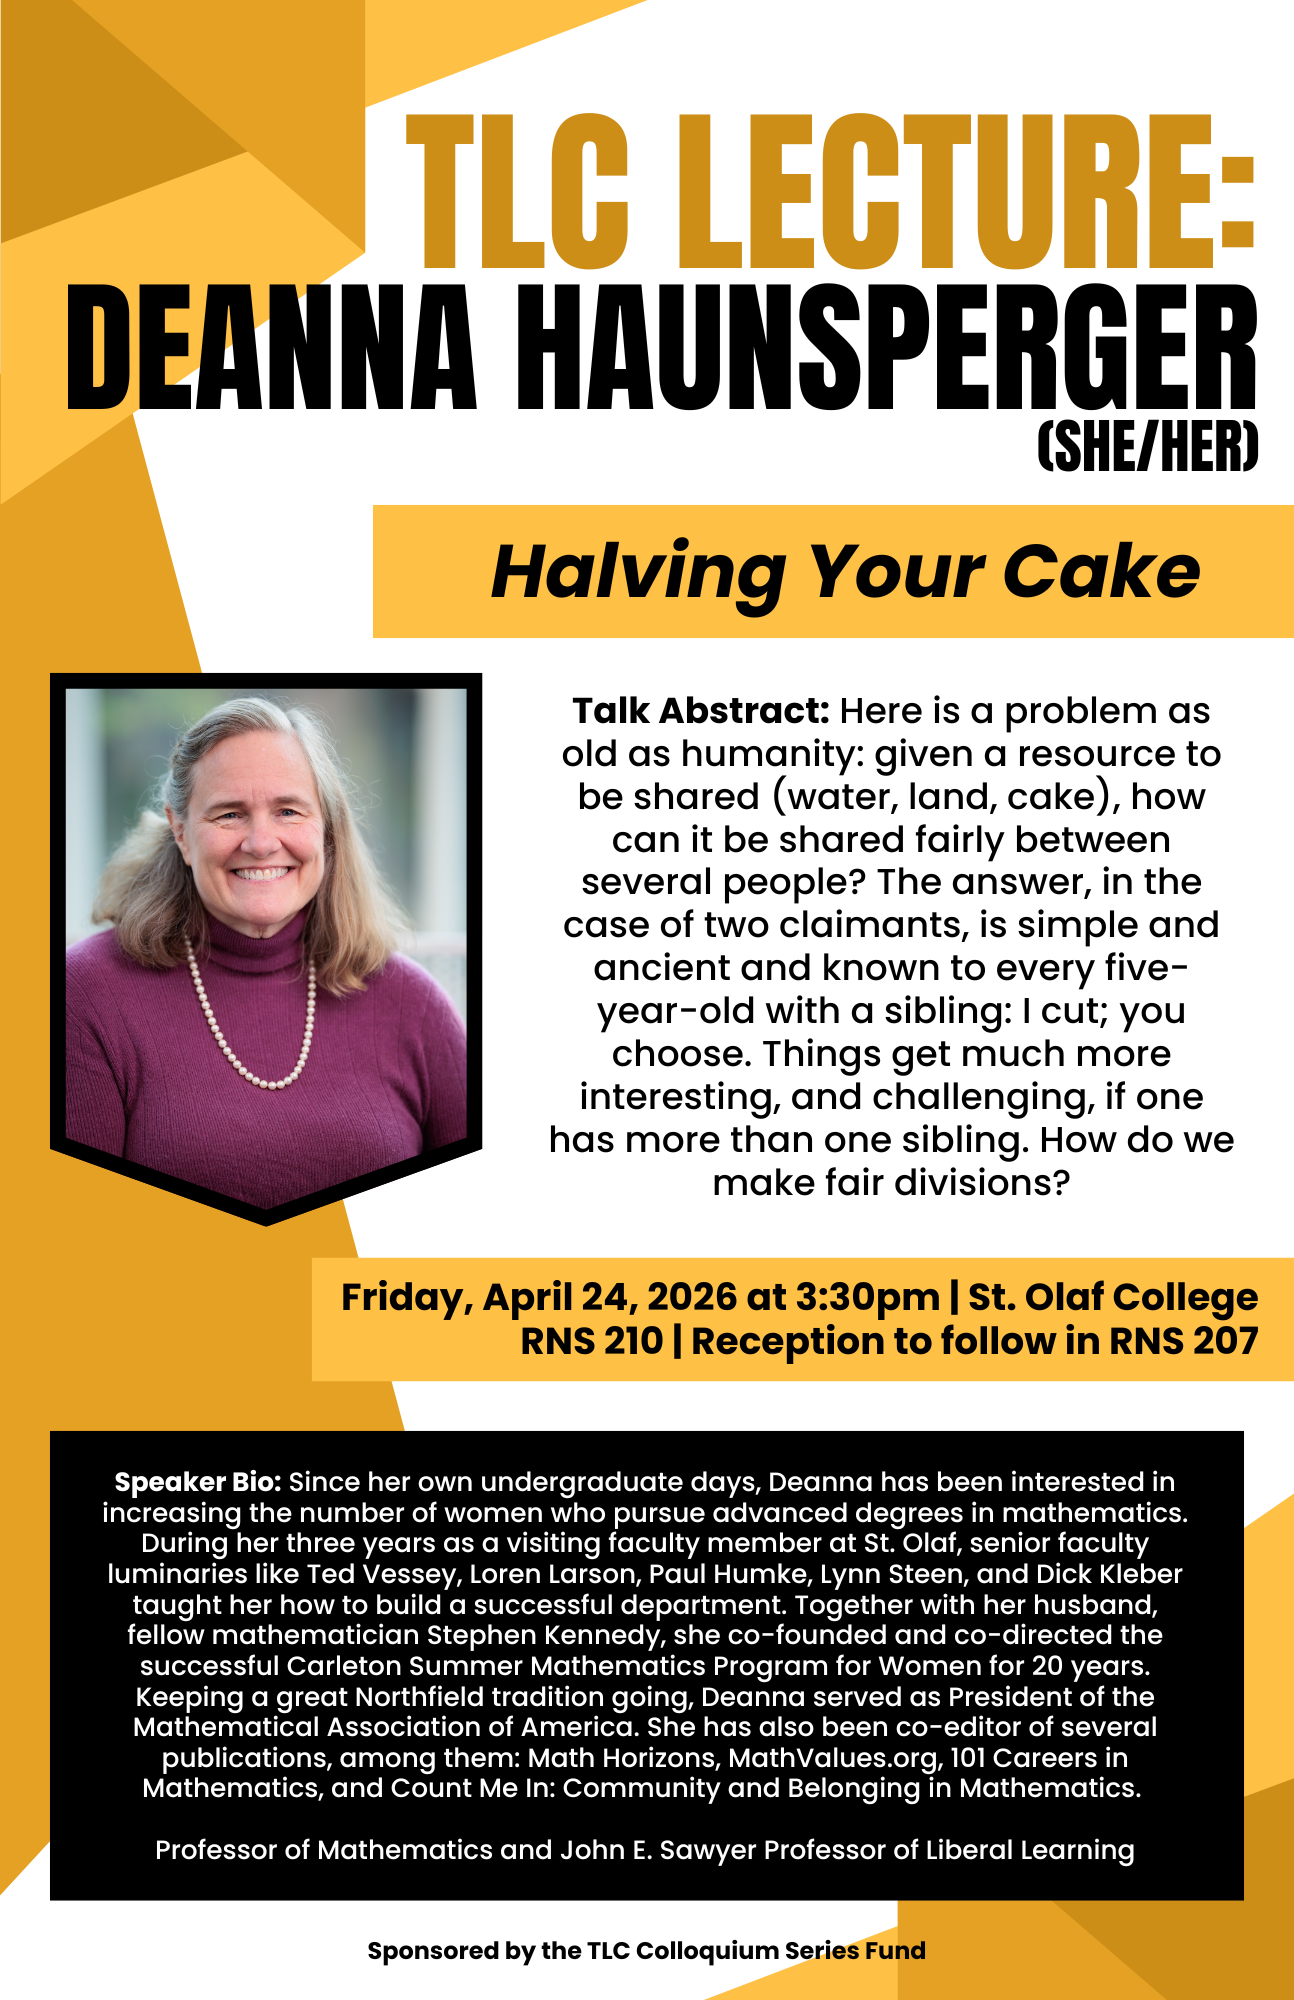
\includegraphics[height=0.95\textheight]{images/TLC Lecture Deanna Haunsperger.png}
\end{center}


\begin{center}
    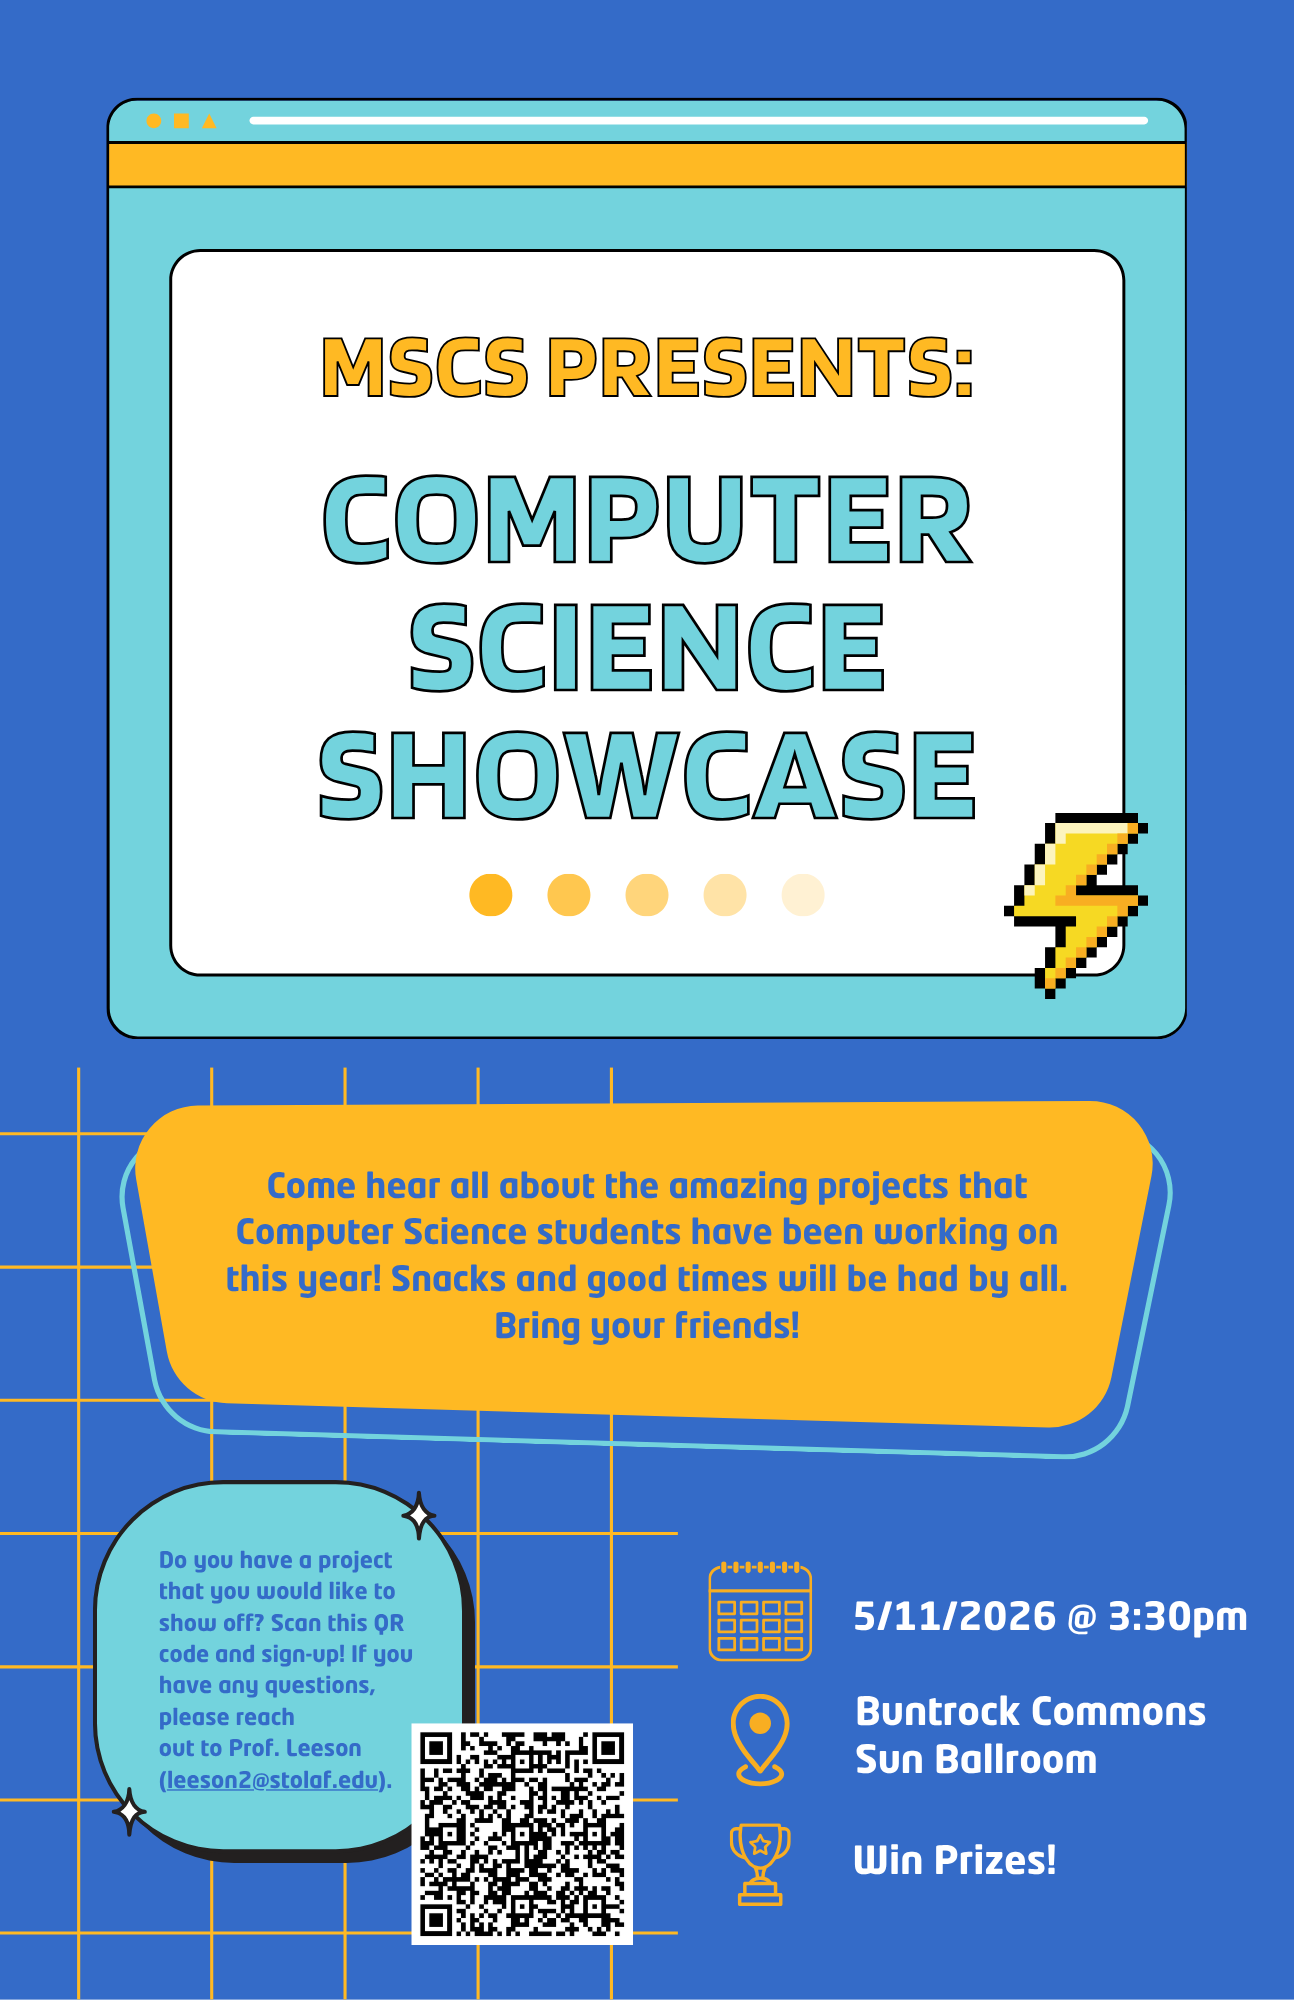
\includegraphics[height=0.95\textheight]{images/Computer Science Showcase (1).png}
\end{center}


\begin{center}
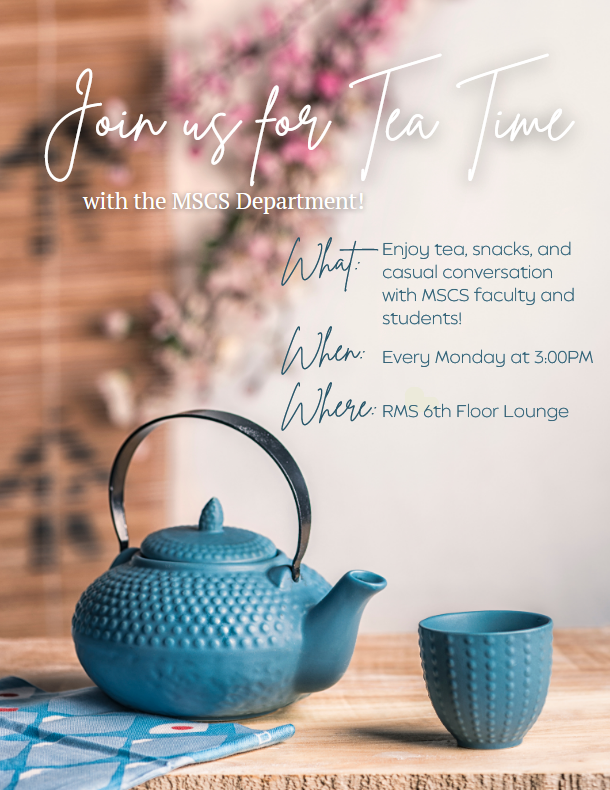
\includegraphics[width=0.9\textwidth]{images/Tea Time Poster.png}
\end{center}

\noindent{To submit an article, event, or anything else for publication in the Mess, email messeditor@stolaf.edu. Visit \href{https://wp.stolaf.edu/mscs/mscs-mess/}{http://wp.stolaf.edu/mscs/mscs-mess/} for a digital archive of previous MSCS Mess issues.}\\
	
\hfill Nima Dahir, Editor
	
\hfill Kyle Salois, Faculty Advisor


 

\end{document}